\documentclass[sigconf]{acmart}
\renewcommand\thesection{\Roman{section}}
\usepackage{algorithm}
\usepackage{algpseudocode}
\usepackage{fancyhdr}

\pagestyle{fancy}
\fancyfoot[L]{Authorized licensed use limited to: Indian Institute of Technology Dharwad. Downloaded on August 22, 2024 at 05:23:16 UTC from IEEE Xplore. Restrictions apply.}

\AtBeginDocument{%
  \providecommand\BibTeX{{%
    Bib\TeX}}}

\setcopyright{acmlicensed}
\copyrightyear{2018}
\acmYear{2018}
\acmDOI{XXXXXXX.XXXXXXX}

\acmConference[Conference acronym 'XX]{Make sure to enter the correct
  conference title from your rights confirmation emai}{June 03--05,
  2018}{Woodstock, NY}

\acmISBN{978-1-4503-XXXX-X/18/06}

\begin{document}

\title{Temperature-Aware Memory Mapping and Active\\Cooling of Neural Processing Units}

\author{%
    \large Vahidreza Moghaddas$^*$, Hammam Kattan$^\dagger$, Tim Bücher$^\dagger$, Mikail Yayla$^*$, Jian-Jia Chen$^{*§}$, and Hussam Amrouch$^{\dagger\ddagger\mathparagraph}$\\
    \textit{\large TU Dortmund University$^*$, University of Stuttgart$^\dagger$, Lamarr Institute for Machine Learning and Artificial Intelligence$^§$}\\
    \textit{\large AI Processor Design, Technical University of Munich$^{\ddagger}$, Munich Institute of Robotics and Machine Intelligence$^{\mathparagraph}$}\\
    \large Corresponding author: vahidreza.moghaddas@tu-dortmund.de
}

\renewcommand{\shortauthors}{Trovato et al.}

\renewcommand{\abstractname}{}
\begin{abstract}
    \textit{\textbf{Abstract}}---\textbf{Neural processing units (NPUs) have become indispensable for meeting the high computational demands of deep neural networks (DNNs). They provide a very efficient solution, thanks to having a huge MAC array that enables massive parallelism. Nevertheless, such an architecture exhibits excessive on-chip power densities leading to a localized hot-spot that seriously heats its surroundings. This work demonstrates how the on-chip temperatures induced by the MAC array create a spatial thermal gradient through the on-chip SRAM memory. This makes the memory regions sensitive to different error probabilities ($P_{error}$), leading to significant accuracy drops when DNNs are being executed. To surmount this challenge, we employ on-chip superlattice thermoelectric (TEC) cooling devices that effectively reduce the memory temperature. Although scaling the memory voltage makes SRAM cells more sensitive to errors, it significantly decreases the leakage power, which compensates for the power consumed by the incorporated TEC devices. Furthermore, operating the SRAM at a lower voltage and temperature substantially increases its lifetime because voltage and temperature are key stimuli of transistor aging. By running multi-physics simulations using commercial finite-element tools and SPICE simulations for the 14nm FinFET technology, we accurately derive the relation between the $P_{error}$ in different memory regions and the corresponding cooling cost. We then propose a three-stage temperature-aware layer-wise memory mapping that exploits different degrees of the sensitivity of NN layers to errors towards maximizing the DNN accuracy while minimizing the cooling cost. Experimental results reveal that our method notably improves the DNN accuracy compared to existing temperature-oblivious memory mapping.}
    \textbf{Index Terms—Thermal management, Neural processing unit (NPU), Thermoelectric cooling (TEC), On-chip memory}
\end{abstract}

\maketitle

\section{Introduction}
A In the past decade, deep neural networks (DNNs) have significantly improved the accuracy of neural networks (NNs). However, running NN applications on general-purpose CPUs is inefficient (in terms of energy and performance) due to the large number of multiplication-accumulation (MAC) operations required to calculate the sum of products of the neurons’ inputs. Custom neural network accelerators are therefore necessary to meet the increasing computational demands. This prompted Google to design and fabricate its first generation of NPUs known as tensor processing unit (TPU), which were deployed in its data centers in 2015, revolutionizing DNN accelerators. TPUv1 can speed up DNN inference by 15-30X with 30 80X less energy consumption than conventional CPUs and GPUs \cite{ref1}.
 
 \begin{center}
     {979-8-3503-1175-4/23/31.00 ©2023 IEEE}
 \end{center}
 
 This breakthrough has motivated other companies to develop their own NPUs, such as Tesla’s full self-driving (FSD) com puter, which comprises two NPU chips in dual configuration, each with 32MB of on-chip SRAM and 96 96 MAC units \cite{ref2}. TPUv1 features 256 256 MAC units with 24MB SRAM, while subsequent generations of TPUs have varying MAC units and/or different on-chip SRAM sizes \cite{ref3}. Nevertheless, having a large number of MAC units in a limited and confined area of the die has reliability consequences. Amrouch et al. in \cite{ref4} showed that even with maximum air cooling, the power density of a 128 128 MAC array can skyrocket to even above 300W/cm2, violating the critical temperature of the chip. Furthermore, in 2018, Google reported that they switched to liquid cooling for their TPUv3 due to its extreme on-chip power density [3]. However, liquid cooling necessitates its own maintenance, cooling infrastructure, and consumes a significant amount of power [3]. 
 
 With the advent of thin-film superlattice thermoelectric cool ing (TEC) devices that can be integrated on top of the silicon die, fine-grained active cooling is now possible \cite{ref5}. Controlled active cooling allows cooling specific region(s) of the die only when needed. These devices can pump heat out of the die with significant heat dissipation of up to 1300W/cm2, as experimen tally demonstrated \cite{ref6}. In [4], a hybrid method is employed for thermal management in NPUs using active on-chip TEC, frequency scaling, and precision scaling. However, the method is only used for the inference of DNNs. Considering NPU for both inference and training, \cite{ref7} explores the design space of Google TPUv3 using Negative Capacitance FET (NCFET) for the MAC array to minimize the TEC cost. Nevertheless, in both papers TEC is considered for the entire die, and the effect of the high power density of the MAC array on the on-chip SRAM memory is not considered. Reagen et al. in \cite{ref8} developed a fault injection framework and explored the resilience of DNNs to errors across different models. Another study proposed software-level error-aware training to tolerate voltage overscaling SRAM errors \cite{ref9}. The robustness of different quantization schemes and error training against low-voltage induced random bit errors has been studied in \cite{ref10} for DNN accelerators with quantized weights stored in SRAM. However, this work assumes the same probability of bit error for the entire memory, while in another work the voltage of different regions of DRAM is scaled down non-uniformly to save energy \cite{ref11}. Notably, neither study considered the impact of high power density of the MAC array on the on chip memory, nor did they explore the use of active cooling.

\textbf{Transistor aging} due to Bias Temperature Instability (BTI) and Hot-carrier Injection (HCI) phenomena is the major relia bility concern for circuit designers. This is due to the profound impact on the circuit performance degradation over time, which may unpredictably, lead to catastrophic timing errors. Both BTI and HCI have a very strong dependency on voltage and temperature. On-chip SRAM memories are one of the prime sources of failures in SoCs because they are powered on continuously throughout the entire lifetime and hence they considerably suffer from aging. Transistor aging manifests itself as drift in the electrical parameters such as Threshold Voltage (VT) \cite{ref12}. This reduces the resiliency of SRAMs against noise and hence errors during read operations start to appear. 

\textbf{Problem and key goals:} In this work, we address the problem of efficiently mapping the NN parameters in on-chip memory for NPUs. We aim to investigate the impact of the high power density of the NPU’s MAC array on the nearby SRAM memory, which results in different probabilities of errors ($P_{error}$) across the memory regions. This exposure to varying error probabilities poses a significant challenge. To tackle this, we employ localized on-chip TEC specifically tar geting the SRAM memory regions. However, employing such active cooling comes with additional power costs. Nevertheless, operating the SRAM memory at a scaled voltage of 03V instead of 07V provides substantial power savings, which can compensate for, if not entirely offset, the extra cooling costs. Note that: (1) Apart from power savings, there is also a significant mitigation of transistor aging, leading to a significant improvement in SRAM reliability. (2) Operating the SRAM at a lower voltage, however, results in higher $P_{error}$. Therefore, our research explores the effective utilization of TECs to compensate for accuracy loss caused by temperature-induced memory errors while minimizing the associated cooling costs. 

\textbf{In short}: We propose a three-stage layer-wise on-chip memory mapping approach for NPUs that maximizes accuracy and minimizes cooling cost by taking into account the varying degrees of robustness of different NN layers to errors. Our approach is orthogonal to any quantization schemes and/or NPUs, and similar results are anticipated. 

\textbf{Our novel contributions within this paper are as follows:} (1) Investigating the impact of MAC array of NPU on the nearby on-chip SRAM memory that creates a spatial thermal gradient through the memory. \\ (2) Integrating active on-chip cooling and memory mapping to maximize the accuracy and minimize the cooling cost.

\begin{figure}[t] % 't' for top
    \centering
    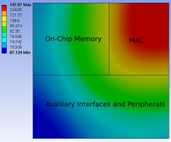
\includegraphics[width=0.25\textwidth]{Figures/Picture1.jpg} % Adjust the width as needed
    \caption{Thermal gradient of TPUv1 when MAC array is hot.}
    \label{Thermal gradient of TPUv1 when MAC array is hot.}
\end{figure}

\section{SYSTEM MODEL AND ASSUMPTIONS}
\textit{A. NPU Thermal Model}

In this work, for the NPU model, we adopt the Google TPUv1 chip. The floorplan is obtained from [1] and consists of a systolic array that occupies around 24\% of the total chip, on chip SRAM memory occupies around 29\% and the remaining part is used for auxiliary management area (I/O, PCIe, periph eral, control, etc.) which occupies around 47\%. The thermal Fig. 1: Thermal gradient of TPUv1 when MAC array is hot. model is performed using commercial ANSYS tool flows that offer accurate multi-physics simulations using finite element methods. In the assumed thermal model, the TPU chip is mounted on top of a printed circuit board (PCB) and is located underneath a cooling unit that consists of a heatspreader, a heatsink, and a fan. A thin layer of thermal interface materials is sandwiched between the TPU silicon die and the heatspreader. Fig. 1, shows how the high temperature of the MAC array creates spatial thermal gradient and affects the on-chip memory (see Section IV-A for simulation setup). Since different memory regions operate under different temperatures, this makes the memory regions susceptible to different probability of errors.

To model the superlattice thin-film TEC, we adopt the proposed structure in [5], [6]. Each TEC module consists of 3 3 thermoelectric couples and has a total surface area of 175mm 175mm. Several TEC modules are implemented to fully cover the entire on-chip SRAM area. The TEC modules have been integrated inside the thermal interface layer to provide effective cooling to the silicon die while avoiding an increase in thermal resistance. When the TEC device is fed with current, a temperature difference between the upper and lower side is formed. The complex interaction between the full system (i.e., PCB, silicon die, heat spreader, heat sink, etc.) and the cooling effects induced by the TEC are accurately captured by the finite element simulations performed by ANSYS. Furthermore, any side effects caused by Joule heat induced inside the TEC will also be captured by the finite element simulations. In order to model the relation between the cooling cost and the corresponding temperature reduction, we sweep the current from 0A all the way up to 6A with a step of 05A. For every current step, we obtain the entire thermal map of the die from the thermal simulation. Then, we calculate the temperature reduction and the corresponding cooling power.\\

\noindent \textit{B. Modeling Error Probability in SRAMs under Voltage and Temperature Effects} 

To accurately model the probability of errors in SRAM cells, we employed SPICE simulations. First, we calibrated the industry-compact model for the FinFET technology (BSIM CMG)toreproduce measurement data from Intel 14nm FinFET. Then, we built a 6-T SRAM cell consisting of two coupled inverters and two access transistors. To capture the impact of process variation of n-FinFET and p-FinFET transistors, we also calibrated the variation against variability data from the same technology node (i.e., Intel 14nm FinFET). Then, we performed Monte-Carlo simulations for the SRAM circuit, in which we measured the transfer characteristics to extract the so-called butterfly curve. This enabled us to compute the static noise margins for both hold and read operations. To obtain sufficient statistical information, we performed 10000 SPICE simulations, providing us with the Hold Noise Margin (HNM) and Read Noise Margin (RNM) distributions. When the distribution crosses the thermal noise which is defined as 26mV, a bit-flip in the SRAM cell occurs. In practice, using the probability density function of the obtained HNM and RNM distributions along with the threshold at which failures occur, the $P_{error}$ of SRAM is then calculated. The impact of temperature on the underlying transistors and hence on the SRAM circuits is accurately captured by the physics-based models within the industry-standard compact model (BSIM-CMG) that we have calibrated against measure ments. We repeated the performed Monte-Carlo simulations for different temperature steps, starting from room temperature (25°C) all the way up to the maximum temperature of 125°C. Afterwards, we did the aforementioned Monte-Carlo analysis for the reduced/scaled voltage (03V) instead of the nominal voltage (07V). In practice, decreasing the voltage reduces the ON current of pFinFET and nFinFET transistors, affecting the HNM and RNM distributions by shifting them considerably towards the thermal noise limit where errors occur. This, in turn, manifests itself as a significant increase in the probability of errors that the SRAM cells will exhibit.\\

\noindent \textit{C. Neural Network Model}

The proposed method in this paper is not limited to any specific neural network (NN), and we provide a general approach to deal with high temperatures that affect memory and degrade the performance of NNs. However, since in most neural processing units (NPUs), quantization is normally applied, in our work, we also consider quantization. Notably, we do not intend to propose a novel quantization and/or exercise state-of-the-art quantization schemes; rather, we use a straightforward quantization to present our method.

\textbf{Quantization: }In this work, we use a uniform-asymmetric quantization scheme. Assume a quantization scheme \( R_Q \), where \( Q \) is a set with a finite number of levels, which we denote here as ordered \( Q = q_1, \ldots, q_L \), where \( q_v < q_{v+1} \) for \( 1 \leq v < L \). We define the number of bits for quantization as \( n_q \), which allows \( L = 2^{n_q} \) quantization levels. Let the value to be quantized be \( x_f \), then the quantized output value \( x_q \) is obtained as:

\[
x_q = \text{round}\left((x_f - \text{min}_{xf}) \frac{2^{n_q} - 1}{\text{max}_{xf} - \text{min}_{xf}}\right) \tag{1}
\]

The values \(\textit{min}_{xf}\) and \(\textit{max}_{xf}\) denote the minimum and maximum values that require quantization. In evaluations, we quantize all parameters of the neural network (NN) to 4 bits, similar to previous studies that also included low-bit weight quantization \cite{ref13}.

\textbf{Training: }For regular NNs, stochastic gradient descent (SGD) is employed with mini-batches. Assume that the training data is described as \( D = \{(x_1, y_1), \ldots, (x_I, y_I)\} \) with \( I \) samples, where \( x_i \) are the inputs, \( y_i \) are the labels, and \( L \) is the loss function. The objective of training is to find a solution for the optimization problem: \(\text{argmin}_W \frac{1}{I} \sum_{(x,y) \in D} L(F_W(x), y)\), using a mini-batch SGD strategy to compute the gradients by backpropagation. Here, \(F_W(x)\) denotes the forward pass function of the NN with learnable parameters \(W\). In the training of quantized neural networks (QNNs), we employ the same procedure, but the weights and biases are quantized during the forward pass of the training phase. In this way, the NN is trained with quantization and can achieve high accuracy despite the limited number of levels. This approach is often referred to as quantization-aware training in the literature [13].

\section{OUR PROPOSED METHOD}

Our layer-wise temperature-aware memory mapping consists of three main steps. In the first step, we determine the sensitivity of each NN layer to errors and use this information to identify the optimal mapping configuration of NN layer parameters to memory regions. Next, we improve the accuracy through error aware training. Finally, we use heuristics to identify the power efficient cooling configuration that meets the target accuracy during the cooling stage.

\textit{A. Profiling and Mapping Stage} 

The goal of this stage is to identify the best way to assign NN layers to different regions of on-chip memory, by taking into account their error sensitivity. We perform error sensitivity analysis of the layers through a per-layer approach. Specifically, we inject faults into each layer and measure the resulting accuracy. By repeating this process for all layers, we can identify the layer(s) that have the most impact on the overall output accuracy. This analysis can be carried out in O(n) iterations of testing, where n is the number of NN layers. After the per layer sensitivity analysis is done, we adopt a greedy approach to assign less error-tolerant layers to more reliable regions of on-chip memory. We assume that each memory region can accommodate at least one layer, and each layer can be mapped to only one region. 

\textit{B. Error Training Stage} 

If the target accuracy cannot be achieved in the previ ous stage, we proceed to train the NN in the presence of temperature-induced errors. As discussed in Section II, the thermal gradient created by the MAC array on the on-chip memory results in different regions having different $P_{error}$ values. 

To adapt the NN to these errors and improve its accuracy, we first use the method described in the profiling stage to assign less error-tolerant layers to more reliable memory regions. Then, during the forward pass of the training procedure (similar to [9]), we inject the corresponding $P_{error}$ values of the memory regions into the layers. This way, the NN can learn to better handle the errors and achieve higher accuracy. 

\textit{C. Power-Efficient Region-Wise Active Cooling }

On top of the two previous steps, we further use TEC devices as active on-chip cooling. We consider regions (columns) in on-chip memory, each of which is covered with TECs, where we have control over each of the TEC regions, i.e. we can determine when and by how much power (cooling cost) should TECs be turned on to dissipate the heat per region. We only consider active cooling that does not lead to Joule heating domination. This means that the cases where increasing the cooling cost leads an increase in temperature/probability of errors are disregarded. Therefore, minimizing the cooling cost under the different probability of errors is monotonic for each region.

Algorithm 1 shows our proposed method. We consider a \\ $\textit{cooling\_cost}_{r \times k}$ matrix, which includes \( k \) cooling power steps consumed for each of the \( r \) regions in increasing order. First, we use the most power-consuming active cooling configuration for all regions. The cooling configuration array keeps track of the column index of the cooling cost matrix for each region (Lines 2-5). Then, if the target accuracy fails to satisfy in this case, the algorithm ends with an error (Line 8). If not, the algorithm goes through a relaxation stage, where it tries to find a power-efficient cooling configuration by reducing the cooling power of each region to its previous power step.

In the relaxation stage (Lines 10-18), we start with a viable configuration, where every region is cooled down with the maximum cooling capacity and tagged as \textit{eligible} for relaxation. Next, we choose a region for relaxation based on a heuristic (either LSF or LSEF which is discussed later) and decrease its cooling power by one step. If this new configuration can also meet the target accuracy, we continue finding more power-efficient configurations; otherwise, we backtrack to the previous configuration and the selected region is tagged as \textit{not eligible} (Lines 15-16). Finally, when there is no eligible region for relaxation, the algorithm terminates and returns the cooling configuration, which shows which TECs should be switched on with what cooling power. The two heuristics that we consider in our work are as follows:

\textbf{Largest Savings First (LSF):} We select the region that provides the largest cost savings when its cooling power is reduced (or relaxed) by one step in the cooling cost matrix. In other words, for region \( i \) (\( 1 \leq i \leq r \)), if the current configuration is column \( j \) in the cooling cost matrix, then the region with the largest \( \Delta C \) is opted, where:

\[
C = \textit{cooling\_cost[i,j]} - \textit{cooling\_cost[i,j-1]} \tag{2}
\]

\textbf{Largest Savings-Error Ratio First (LSEF):} We choose a region for relaxation that provides the largest cooling cost savings but with the least \( P_{\text{error}} \) coverage; in other words, the one that gives the largest cost-error ratio when relaxed to the previous step in the cooling cost matrix is selected as:

\[
\frac{\Delta C}{\Delta E} = {\frac{\textit{cooling\_cost}[i,j] - \textit{cooling\_cost}[i,j-1]}{P_{\textit{error}}[i,j-1] - P_{\textit{error}}[i,j]}} \tag{3}
\]

Noteworthy, since we have at most \( rk \) iterations of relaxations, the complexity of the proposed Algorithm 1 is of \( O(rk) \) iterations of testing.

\textit{D. Overview of our Proposed Algorithm}

To conclude this section, we provide an overview of our proposed algorithm for temperature-aware memory mapping in Algorithm 2. The algorithm involves a profiling stage, followed by a mapping stage, and then potentially an error training stage, followed by an active cooling stage as a last resort. The profiling stage is performed using a per-layer sensitivity analysis, as described in Section III-A (Lines 1-5). Once the sensitivity analysis is complete, the layers are sorted in non-increasing order of sensitivity (Line 6), and then mapped to memory regions in a greedy manner, starting with the most reliable memory regions (Lines 7-12). If a layer can be accommodated in a memory region, it is assigned to that region; otherwise, the algorithm moves on to the next region (Lines 9-10). If the target accuracy is not met, the algorithm proceeds to the error training stage (Lines 13-15). In this stage, the model is trained with the probability of errors with the goal of improving accuracy. If further accuracy compensation is required, the algorithm proceeds to the active cooling stage (Lines 19-23), which is described in Algorithm 1. If active cooling is unsuccessful, the algorithm returns with no solution to achieving the target accuracy (Lines 24-26).

\begin{algorithm}[t]
\caption{Power-Efficient Region-Wise Active Cooling}
\begin{algorithmic}[1]
\Procedure{active\_cooling}{model}
    \For{$i \gets 1$ to $R$}
        \State $cooling\_config[i] \gets k$
        \State $eligible[i] \gets 1$
    \EndFor
    \State $accuracy \gets test(model)$
    \If{$accuracy < target\_accuracy$}
        \State \textbf{return} error
    \EndIf
    \Repeat
        \State Choose eligible region $i$ for relaxation according to LSF or LSEF
        \State $cooling\_config[i] \gets cooling\_config[i] - 1$
        \State $accuracy \gets test(model)$
        \If{$accuracy < target\_accuracy$}
            \State $cooling\_config[i] \gets cooling\_config[i] + 1$
            \State $eligible[i] \gets 0$
        \EndIf
    \Until{$\forall j, eligible[j] = 0$}
    \State \textbf{return} $cooling\_config$
\EndProcedure
\end{algorithmic}
\end{algorithm}

\section{EVALUATION}
\textit{A. Experiment Setup}

In our experiments, we use four datasets, namely Fashion MNIST, SVHN, CIFAR10, and Imagenette, with the details given in Table I. We also employ VGG \cite{ref14} , MobileNetV2 \cite{ref15}, and ResNet \cite{ref16} models adapted to their corresponding datasets. For Fashion MNIST and SVHN, we run the Adam optimizer for 50 epochs, and for CIFAR10 and Imagenette, we run it for 200 epochs with a batch size of 256 and an initial learning rate of $10^{-3}$ for all cases. To stabilize training, we decrease the learning rate by 50\% after every 50 epochs for CIFAR10 and Imagenette, and after every second epoch for SVHN and Fashion MNIST. To run our experiments, we use the PyTorch environment for neural network training and evaluation. PyTorch allows C++ level access to the tensors using custom CUDA kernels, which we use for efficient quantization and fault injections. The bit-flip faults are injected into the weights and biases by creating random numbers for each bit to be flipped. If a random number is smaller than the $P_{\text{error}}$, the bit is flipped. In thermal multi-physics simulations, we use the commercial ANSYS tool (see Section II-A for modeling). A power density of 200 W/cm² is considered for the MAC array, and 30 W/cm² for on-chip memory and the auxiliary components. Moreover, we assume a heat transfer coefficient of 100 W/m²K, which is the highest forced convection of air under the maximum capability of fan-based cooling . With this configuration, the total power of the TPU die reaches 725 W, in which the MAC, SRAM, and auxiliary consume 50 W, 75 W, and 15 W, respectively. In addition, we consider three equal regions (or columns) for the on-chip memory, from the farthest region to the MAC array (Region 1) to the nearest one (Region 3). Noteworthy, the number of regions can be determined based on the physical limitations of TECs and/or the floor plan of the NPU, in addition to the thermal gradient of on-chip memory.

\begin{algorithm}
\caption{Temperature-Aware Memory Mapping}
\begin{algorithmic}[1]
\For{$i \gets 1$ to $n$}
    \State fault injection(layer[$i$], fixed error rate)
    \State accuracy $\gets$ test(model)
    \State sensitivity\_list[$i$] $\gets 1 -$ accuracy
\EndFor
\State Sort layers w.r.t. sensitivity\_list in non-increasing order
\State $r \gets 1$
\For{$i \gets 1$ to $n$}
    \If{map(region[$r$], layer[$i$]) = false}
        \State $r \gets r + 1$
    \EndIf
\EndFor
\State accuracy $\gets$ test(model)
\If{accuracy $<$ target\_accuracy}
    \State train(model, $P_{error}$)
\Else
    \State \textbf{return} mapping
\EndIf
\State accuracy $\gets$ test(model)
\If{accuracy $\geq$ target\_accuracy}
    \State \textbf{return} mapping
\ElsIf{active\_cooling(model) = error}
    \State \textbf{return} mapping with the cooling configuration
\Else
    \State print "no possible solution"
    \State \textbf{return}
\EndIf
\end{algorithmic}
\end{algorithm}

\begin{table}
    \centering
    \caption{Datasets and models used for experiments}
    \begin{tabular}{@{}lcccc@{}}
        \toprule
        Name (Model) & \#Train & \#Test & \#Dim & \#Classes \\ \midrule
        Fashion-MNIST (VGG3) & 60000 & 10000 & (1, 28, 28) & 10 \\
        SVHN (VGG7) & 73257 & 26032 & (3, 32, 32) & 10 \\
        CIFAR10 (MobileNetV2) & 50000 & 10000 & (3, 32, 32) & 10 \\
        Imagenette (ResNet18) & 9470 & 3925 & (3, 64, 64) & 10 \\ \bottomrule
    \end{tabular}
\end{table}

\begin{figure}
    \centering
    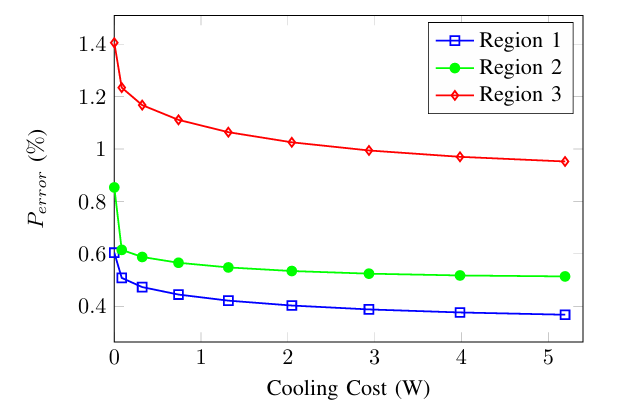
\includegraphics[width=0.45\textwidth]{Figures/Picture2.png} 
    \caption{The effect of active on-chip cooling on the probability of
 errors ($P_{error}$) for the 3 on-chip memory regions. Cooling cost is
 represented by the total power consumed by the TEC devices in Watt.}
    \label{The effect of active on-chip coolingon the probabilityof
 errors (Perror) for the3on-chipmemory regions. Coolingcost is
 representedbythetotalpowerconsumedbytheTECdevicesinWatt.}
\end{figure}

\begin{figure}
    \centering
    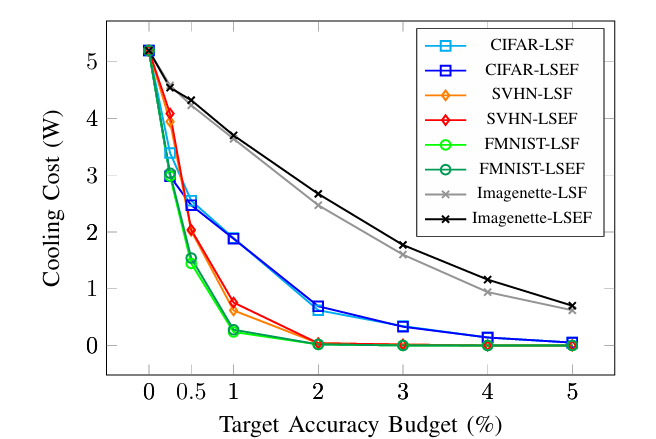
\includegraphics[width=0.45\textwidth]{Figures/Picture3.png} 
    \caption{The effect of different target accuracy budgets on the
 cooling cost using LSF and LSEF heuristics.}
    \label{Theeffect ofdifferent target accuracybudgetson the
 coolingcostusingLSFandLSEFheuristics.}
\end{figure}

\vspace{3em}
\noindent \textit{B. The Effect of Active Cooling on the Probability of Errors}

In Fig. 2, the effect of using active on-chip TEC cooling on the \( P_{\text{error}} \) of the different memory regions is shown. The values for \( P_{\text{error}} \) in this figure are the average of each region. Due to the spatial thermal gradient created by the MAC array through the on-chip memory, the temperature and the corresponding \( P_{\text{error}} \) for different memory regions have a considerable difference. Hence, the region in the immediate neighborhood of the MAC (Region 3) is hotter, leading to a higher \( P_{\text{error}} \). By paying more cooling cost, the \( P_{\text{error}} \) decreases for all the regions; however, it is noteworthy to note that beyond the values for the cooling cost in Fig. 2, since Joule heating dominates and leads to higher temperatures, it is not considered in the evaluations. This is also the reason why the trend in the figure starts with a steep decline and then the slope of the curves gradually plateaus.

\noindent \textit{C. The Effect of Target Accuracy on Cooling Cost}

We consider the following set of target accuracy budgets: 0, 2, 5, 10, 12, 34, 5 percentage below the maximum feasible accuracy achieved through maximum active cooling: 91.43\% (SVHN), 90.43\% (Fashion-MNIST), 80.46\% (CIFAR10), and 56.36\% (Imagenette). In Fig. 3, the two heuristics introduced in Section III-C for active cooling are compared for different target accuracies. Each data point in the figures corresponds to the average of 100 experiments. For the Fashion-MNIST dataset, no active cooling is necessary for target accuracy budgets 3, 4, 5\%. Similarly, for SVHN, the previous stages of our proposed method can meet the accuracy demands for target accuracy budgets 4, 5\%. However, for CIFAR10 and Imagenette, active cooling is essential for all target accuracies. On using the TEC devices efficiently, the greedy cost savings heuristic (LSF) performs slightly better than LSEF.

In Fig. 4, we present the accuracy results obtained with and without active cooling for different datasets, using the LSF heuristic. Temperature-oblivious in the figure represents the memory mapping that is done irrespective of the thermal profile of memory regions (similar to [10]). Profiling and Error Training represent the two stages of our method. We consider two scenarios for active cooling: (1) with 1\% target accuracy budget denoted as Active Cooling, and (2) with the maximum cooling cost (519 W) denoted as Max Cooling. Finally, No Error is given as a reference for the scenario where there are no errors in the memory.

For the CIFAR10 dataset, our method can improve the accuracy from 21.6\% in temperature-oblivious mapping to 79.8\% in active cooling (18 W), and above 80\% through the maximum cooling. For the Imagenette dataset, the accuracy cannot rise above 46\% without using active cooling even under temperature-aware mapping and error training. For the Fashion-MNIST dataset, the values that are subject to errors are more error tolerant compared to CIFAR10; even in temperature-oblivious mapping, the accuracy is as high as 74\%. Through passing the first two stages of our method, the accuracy reaches 88\%. If the target accuracy is met until this point, there is no demand to incur active cooling; however, higher target accuracies are only viable via active cooling. Moreover, for the SVHN dataset, while in the oblivious mapping the accuracy can be as low as 27\%, only by consuming 0.62 W, the accuracy can rise to over 90\%.

\textbf{On the Cost of Cooling Power Overhead: }To estimate the obtained power saving via memory voltage scaling, we employ the state-of-the-art version of CACTI (i.e., FN-CACTI) \cite{ref17}. We model in FN-CACTI, 24 MB memory (mimicking the memory size in the TPUv1 chip) at two different voltages (0.7 V and 0.3 V). We then perform simulations for these two scenarios. An 83\% reduction in on-chip memory power is observed, which is attributed to the exponential dependency of leakage power as well as the quadratic dependency of dynamic power on voltage. This reduces the power consumed by on-chip SRAM by around 62 W. Such obtained power saving compensates and cancels out the additional power cost needed for the TEC cooling even under the worst case in which 519 W is requested.

\textbf{On the Reliability Improvement: }Note that operating SRAMs at lower voltage and temperature results in a significant improvement in reliability. To evaluate this improvement, we employ state-of-the-art physics-based aging models that are calibrated against industrial measurements for the FinFET technology [12] in order to accurately estimate the aging induced \( V_T \). We consider two scenarios: (i) in the absence of our proposed cooling in which transistors operate at 0.7 V, 97.5 °C, and (ii) in the presence of our proposed cooling in which transistors operate at 0.3 V, 80.8 °C. For a 10-year lifetime, the obtained results demonstrate that our cooling solution reduces the aging-induced \( V_T \) from 34.32 mV (obtained from scenario (i)) down to merely 8.23 mV (obtained from scenario (ii)), which substantially improves (76\%) the SRAM reliability for the entire lifetime.

\begin{figure}
    \centering
    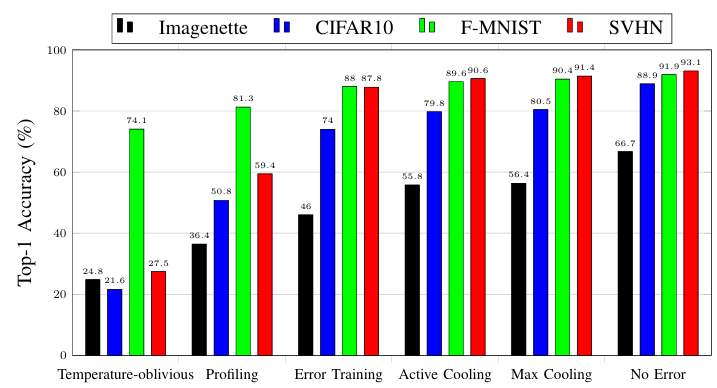
\includegraphics[width=0.45\textwidth]{Figures/Picture4.png} 
    \caption{Compensating accuracy loss at different stages of the
 proposed method for different datasets. The power consumption
 in active cooling for Imagenette, Cifar10, FMNIST, and SVHN
 are 37W, 18W, 024W, and 062W respectively.}
    \label{Compensating accuracy loss at different stages of the
 proposed method for different datasets. The power consumption
 in active cooling for Imagenette, Cifar10, FMNIST, and SVHN
 are 37W, 18W, 024W, and 062W respectively.}
\end{figure}

\section{Neural Processing Units}

Neural processing units are specifically designed to accelerate neural network applications. At the heart of these accelerators is a huge MAC array that speeds up the multiply-accumulate operations. In this work, we demonstrate that the power density of the MAC array has a significant impact on the nearby on-chip SRAM memory for Google’s TPU. This effect creates a thermal gradient through the memory, making its regions sensitive to the different probability of errors. Super lattice thermo electric cooling (TEC) as an active cooling can efficiently cool down the on-chip memory and compensate for the accuracy loss caused by the high power density of the MAC. The evaluations show that our temperature-aware memory mapping and active cooling method can be efficiently used to achieve higher target accuracies.

\section*{ACKNOWLEDGMENT}

This paper has been supported by Deutsche Forschungsgemeinschaft (DFG) within the project OneMemory (project number 405422836), the SFB 876 (project number 124020371), and project ACCROSS (428566201, AM 534/3-1).

\bibliographystyle{IEEEtran}
\bibliography{acmart}

\end{document}